%%%%%%% Preambule %%%%%%%%
% !TeX program = xelatex
% !BIB program = biber
% třída dokumentu
\documentclass[12pt,a4paper,hidelinks]{article}

% kvůli písmům a ligaturám (např. --)
% toto je pro XeLaTeX!
\usepackage{fontspec}
\defaultfontfeatures{Mapping=tex-text}
\usepackage{xunicode}
\usepackage{xltxtra}
\setmainfont{Times New Roman}

% nastavení jazyka (kvůli dělení slov, apod.)
% toto je pro XeLaTeX!
\usepackage{polyglossia}
\setdefaultlanguage{czech}

% když polyglossia, fontspec, xltxtra je to xelatex

% rozšíření od AMS na vzorečky
\usepackage{amsmath}
\usepackage{amsfonts}
\usepackage{amssymb}

% definice nové fce
\DeclareMathOperator{\tg}{tg}

%balíček pro \dif
%\usepackage{commath}
%pro rovná řec. písmena
%\usepackage{upgreek}

% potřebujeme na obrázky
\usepackage{graphicx}

% okraje
 \usepackage[left=2cm,right=2cm,top=2cm,bottom=2cm]{geometry}
%\usepackage{a4wide}

% alternativní písma
% \usepackage{kpfonts-otf}
% \usepackage{fourier-otf}
\setmainfont{Times New Roman}


% balíček pro výplňový text (lorem ipsum)
\usepackage{lipsum}

% balíček pro lepší práci s odkazy
\usepackage[unicode]{hyperref}

% balíček pro nastavení odstavců
\usepackage{parskip}
\setlength{\parindent}{2em}
% balíček pro nastavení řádkování
\usepackage{setspace}
\onehalfspacing

% balíček pro rozšíření seznamů
\usepackage{enumitem}
\setlist[enumerate, 2]{label={\alph*)}}
\setlist[enumerate, 3]{label={\roman*)}}

%bal. pro sluč řádků
\usepackage{multirow}

%bal. pro hezčí tabulky
\usepackage[table]{xcolor}
\usepackage{booktabs}

%pro hezčí popisky
\usepackage{caption}
\captionsetup [table]{skip=2pt}

%bal pro sazbu do vícce sloupců
\usepackage{multicol}

%české uvozovky
\usepackage{csquotes}

\usepackage{footnote}
\makesavenoteenv{figure}

% odřezávání rádků
\tolerance=1
\emergencystretch=\maxdimen
\hyphenpenalty=10000
\hbadness=10000

%balíček pro hezčí práci s čísly a jednotkami
%pro příkazy \num{1235456}, \SI{123456}{km} či \SI{30}{\celsius}
\usepackage{siunitx}
\sisetup{locale=DE}

%Numbering věc i guess
\usepackage{chngcntr}
\counterwithin*{section}{part}

%kód
\usepackage{listings}
\usepackage{xcolor}

\definecolor{codegreen}{rgb}{0,0.6,0}
\definecolor{codegray}{rgb}{0.5,0.5,0.5}
\definecolor{codepurple}{rgb}{0.58,0,0.82}
\definecolor{backcolour}{rgb}{0.95,0.95,0.92}

\lstdefinestyle{mystyle}{
    backgroundcolor=\color{backcolour},
    commentstyle=\small\color{codegreen},
    keywordstyle=\color{magenta},
    numberstyle=\tiny\color{codegray},
    stringstyle=\color{codepurple},
    basicstyle=\ttfamily\footnotesize,
    breakatwhitespace=false,
    breaklines=true,
    captionpos=b,
    keepspaces=true,
    numbers=left,
    numbersep=5pt,
    showspaces=false,
    showstringspaces=false,
    showtabs=false,
    tabsize=2
}

\lstset{style=mystyle}

\usepackage{pdflscape}

%balíček pro automatické generování citací
% urldate: formátovaní data citování (položka urladate)
% iso je yyyy-mm-dd
% sorting: způsob řazení citací, none je původní (citované) pořadí
% nty: jméno, název, rok
% style: způsob formátování/zobrazení citace, iso-numeric je čsn iso 690-2 (citace.com + číslované), iso-author title je to stejný, ale pro humanitní (pozn. pod čarou)
% pro přírodní vědy
 \usepackage[urldate=iso, sorting=none, style=iso-numeric]{biblatex}
% pro humanity
% \usepackage[urldate=iso, sorting=nty, style=iso-authortitle]{biblatex}
\addbibresource{Zdroje.bib}

% Autor, název a datum
\author{Vojtěch Hána}
\title{Jednoduchá PC hra}
\date{mnogo}

%%%%%%% Konec preambule = začátek dokumentu %%%%%%%%

\begin{document}
\begin{titlepage}
    \centering
    {\large Gymnázium, Praha 7, Nad Štolou 1}
    \vfill
    {\Large \textsc{Maturitní práce}\par} % \par opraví řádkování
    \vspace{0.5cm}
    {\Huge \textbf{Jednoduchá PC hra}\par} % \par opraví řádkování
    \vfill\vspace{2cm}

    \begin{large}
        \begin{tabular}{>{\raggedleft\arraybackslash}p{7cm}>{\raggedright\arraybackslash}p{7cm}}
            \textbf{Autor práce}: & Vojtěch Hána \\
            \textbf{Vedoucí práce}: & Martin Sourada \\
            \textbf{Třída}: & 6S \\[0.5cm]
            \multicolumn{2}{c}{2022/2023} \\
        \end{tabular}
    \end{large}
\end{titlepage}
\addtocounter{page}{1}

\clearpage

\begin{abstract}
Tato maturitní práce se zabývá procesem vývoje počítačové hry v enginu Unreal. Zaměřuje se nejdříve na průběh vývoje a rozhodnutí, která jej provázela, poté na konkrétních příkladech představuje některé postupy, které lze při vývoji v tomto enginu využít. Dále tato práce ve své praktické části obsahuje autorem vytvořenou videohru, o níž se pojednává v části teoretické a příručku k této hře.

This final thesis deals with the process of developing a computer game in the Unreal engine. It focuses first on the development process and the decisions that accompanied it, then it presents some of the techniques that can be used in the development in this engine using concrete examples. Furthermore, the practical part of this thesis includes a video game created by the author, which is discussed in the theoretical part, and a manual for this game.
\end{abstract}



\clearpage
\thispagestyle{empty}

Prohlášení: Prohlašuji, že jsem maturitní práci vypracoval samostatně, použil jsem pouze podklady uvedené v přiloženém seznamu a postup při zpracování a dalším nakládání s prací je v souladu se zákonem č. 121/2000 Sb., o právu autorském, o právech souvisejících s právem autorským a o změně některých zákonů (autorský zákon), ve znění pozdějších předpisů.

V Praze dne \today

\clearpage
\thispagestyle{empty}
Tímto bych chtěl poděkovat Bc. Martinu Souradovi za vedení práce a užitečné rady, dále Emilii Ďurišové, Marku Hlavovi a Vítu Šeflovi za nedocenitelnou pomoc při testování hry.

\clearpage
%\begin{small}
	\tableofcontents
%\end{small}
\clearpage

\section*{Úvod}
\addcontentsline{toc} {section} {Úvod}
Herní vývoj je prostředí, ve kterém existuje tolik správných způsobů, jak dosáhnout cíle, kolik je vývojářů. Tato práce si nedává za cíl zpracovat do hloubky obecný postup vývoje videohry nebo prezentovat určité postupy jako jediné správné. Pojednává naopak o vývoji konkrétní hry a snaží se přiblížit unikátní okolnosti tohoto vývoje. Toto téma jsem si vybral, jelikož tematika videoher a jejich vývoje je mi blízká, a to jak z pozice pozorovatele, tak případného budoucího vývojáře.

V této práci se také snažím sdělit některé základní informace o programování ve vizuálním jazyce Blueprint.\cite{uedocs:blueprint} Tyto informace jsou podávány prostřednictvím popisu specifických funkcí a způsobů, jak fungují v praxi.

\clearpage

\part{Teoretická část}
\section{Užité nástroje}
\subsection{Engine}
Veřejnosti je přístupno nepřeberné množství herních enginů, každý z nich se svými plusy a mínusy, orientovaný na jiný segment trhu. Například \textit{Unigine}\cite{unigine} exceluje ve velkých scénách díky 64bitovým souřadnicím, zatímco \textit{Clausewitz} je zaměřený na top-down grand-strategy hry.

Jelikož Astra je mým prvním velkým projektem, co se vývoje her týče, bylo pro mne důležité, aby pro zvolený engine byla dostupná rozsáhlá a kvalitní dokumentace a aktivní komunita, na kterou by se bylo možná obrátit v případě potíží. Tím z výběru vypadávají všechny málo známé enginy a také ty, které sice známé jsou, ale většinou na nich vyvíjejí pouze velká studia, jako například \textit{CryEngine}\cite{cryengine}.

Po tomto prvním kroku zbývali dva seriózní kandidáti, a to \textit{Unity}\cite{unity} a \textit{Unreal Engine}\cite{unreal}. Finální volba nakonec padla na novější Unreal Engine 5 (nadále v této práci zkracován UE). Ten se jevil jako lepší volba díky jeho systémům jako je například engine osvětlení Lumen\cite{uedocs:lumen}, který by mi značně usnadnil tvorbu realisticky vypadající grafiky.

\subsection{Další užité nástroje}
UE má ve své základní distribuci zabudováno rozsáhlé množství nástrojů pro tvorbu a nakládání s různými soubory. I přesto bylo v průběhu vývoje nutné využít několik dalších programů:

\subsubsection{GIMP}
GIMP je zkratka pro \enquote{GNU Image Manipulation Program}\cite{gimp}. Jedná se o open-source grafický editor, který umožňuje uživatelům úpravu a vytváření digitálních obrázků Nabízí funkce pro práci s vrstvami, efekty, filtraci, kreslení a malování, retušování apod. Je k dispozici pro operační systémy Windows, Mac a Linux a je dostupný zdarma ke stažení a použití.

Tento program jsem využil na tvorbu některých textur a design prvků uživatelského rozhraní. Oproti konkurenčním programům, jako je např. Adobe Photoshop\cite{photoshop}, jsem GIMP zvolil zejména kvůli předchozí znalosti tohoto programu.

\subsubsection{Audacity}
Audacity\cite{audacity} je volně dostupný audio editor a nahrávací software pro operační systémy Windows, Mac a Linux. Umožňuje uživatelům nahrávat, upravovat a mixovat zvukové soubory v různých formátech a kodecích. Audacity obsahuje mnoho funkcí, jako jsou například úpravy hlasitosti, střihu, normalizaci, změnu rychlosti a změnu výšky tónu. Může být použit pro mnoho různých účelů, včetně nahrávání a úpravy hudby, podcastů, záznamů rozhovorů nebo dokonce nahrávání a úpravu zvukových stop pro videa.

Vzhledem k možnosti upravovat zvukové stopy přímo v UE jsem Audacity užil jen zřídka, a to na úpravu hlasových stop pro postavu hráčovy AI pomocnice a pro přípravu zvukových stop na import převodem na podporovaný kodek. Podobně jako GIMP jsem tento program zvolil na základě předchozí zkušenosti.


\subsubsection{Git}
Git\cite{git} je distribuovaný systém správy verzí, který se používá pro sledování změn v kódu a koordinaci práce více lidí na společném projektu. Je to nástroj, který umožňuje uživatelům ukládat, verzovat a spravovat svůj kód a jeho historii.

Git umožňuje uživatelům pracovat na kopii kódu, kterou si mohou upravovat bez toho, aby se to projevilo na hlavní větvi (tzv. \enquote{master branch}). Poté, co provedou své změny a jsou s nimi spokojeni, mohou je zahrnout do hlavní větve. Git také umožňuje ukládat různé verze kódu v různých větvích, což usnadňuje vývoj a testování nových funkcí nebo náprav chyb. Díky němu je také snadnější zpětné získání předchozích verzí kódu a práce na nich.

Jelikož jsem na projektu pracoval sám, řady z vlastností Gitu jsem vůbec nevyužil. Stejně tak zůstala nevyužitá i možnost vývoje ve více větvích (z důvodu, že jsem dříve nebyl se systémy sledování verzí seznámen), což není optimální.

\subsubsection{Blender}
Blender\cite{blender} je otevřený a zdarma dostupný software pro 3D modelování, animaci a vizualizaci, široce používaný v oblasti filmového a herního průmyslu, architektury, designu a mnoha dalších. Uživatelům umožňuje vytvářet 3D objekty, animovat je, texturovat, osvětlovat a renderovat. Další funkcí Blenderu jsou například simulace fyziky, jako jsou srážky a deformace, simulace tekutin a plamenů apod.

Uživatelé také mohou vytvářet složité animace pomocí animačních klíčů, sledování kamer a světel, a dalších funkcí. Právě tuto konkrétní funkci jsem při vývoji použil, a to na vytvoření krátkého videa s logem hry, které se přehrává, když se hra spouští.
\clearpage

\section{Počáteční cíle}
Celkový koncept hry se během vývoje několikrát změnil. Původní plánování jsem ale provedl s následujícími cíli.
\begin{itemize}
	\item Střílečka z pohledu třetí osoby (\textit{Third-person shooter}), zasazený ve vesmírném prostředí.
	\item Pohybový model hráčovy vesmírné lodě, který umožňuje pohyb po všech šesti osách (tj. 3 osy trojrozměrného prostoru + 3 osy otáčení)
	\item Absence konečného úkolu – hra skončí pouze selháním či přáním hráče
	\item Počítačoví protivníci, kteří se dokáží v prostoru pohybovat stejným způsobem jako hráč a jsou schopni na něj efektivně útočit
	\item Realisticky vypadající (nestylizovaná) grafika
\end{itemize}

Za inspiraci měly sloužit podobné hry, jako například nedávno vydané \textit{Star Wars: Squadrons}\cite{squadrons} a starší \textit{Star Wars: Battlefront II}\cite{bf2} od Electronic Arts nebo \textit{Elite: Dangerous}\cite{elite} od Frontier Developments.

\section{Vývoj}
UE uživatelům nabízí několik předem zhotovených šablon\cite{uedocs:templates}, které obsahují všechny základní nezbytné prvky a dovolují uživatelům pouze rozšiřovat z tohoto funkčního základu. Této možnosti jsem nevyužil, jelikož žádná z nabízených šablon nevyhovovala výše uvedeným požadavkům. Zejména problematická by byla implementace volného pohybu v trojrozměrném prostoru – ve všech šablonách se počítalo s přítomností země a gravitace.

\subsection{3D}
Prvním úkolem pak tedy bylo vytvořit prázdnou úroveň a naprogramovat základní funkce. Původní letecký model z této prvotní fáze byl ovládaný kombinací myši a klávesnice. Klávesnice zajišťovala rotaci okolo vektoru pohybu, zatímco myš zajišťovala stáčení. Loď cestovala neměnnou rychlostí (pokud nedošlo ke kolizi). V úrovni se také vyskytoval jeden \enquote{nepřítel}, který sloužil jako test systému střelby. Nepřítel samotný se nijak nepohyboval ani neútočil. Jediná jeho implementovaná funkce bylo jeho zničení, kdy po určitém počtu zásahů zmizel.

Další verze zaznamenaly několik zlepšení k funkcím hráčovy lodě. Nově hráč mohl změnit rychlost letu v rámci povoleného rozsahu. Zároveň se objevila chyba v zobrazování uživatelského rozhraní, která zůstala dlouhou dobu nespravena. Naopak několik chyb bylo odstraněno, a to převážně v konzistentnosti systému střelby. V neposlední řadě došlo ke změnění osvětlení úrovně a přidání několika překážek v podobě asteroidů.


\subsubsection{Přechod na 2D}
Problém s původní 3D koncepcí se objevil při práci na počítačových protivnících. Bohužel, pathfinding v trojrozměrném prostoru se ukázal jako extrémně obtížný na implementaci, alespoň pro začátečníka. Došel jsem k názoru, že jelikož není možné hru v tehdejší koncepci dokončit, a je tedy nutné změnit cíle Nesmírnou nevýhodou bohužel bylo, že zhruba polovina dosavadní práce tak musela být zahozena. Zůstat mohlo jenom pozadí (tzv. \textit{skybox}) a modely lodí. Veškerá logika a kód ale musely být kompletně přepsány.

Jako první bylo nutné určit, do jakého žánru bude Astra spadat. Z důvodu osobní preference tohoto žánru jsem nakonec zvolil tzv. \textit{\enquote{top-down shoot-em-up}}, konkrétně jeho podžánr \textit{\enquote{bullet hell}}.

Tyto hry mají několik identifikujících znaků. Rozeberme si proto jednotlivé pojmy.

\enquote{Top-down}, doslovně \enquote{zezhora dolů}, značí hru, ve které je kamera fixně umístěna nad herním polem, a ve které se hráč pohybuje po obrazovce nezávisle (typicky po osách X a Y, ne však do hloubky).

\enquote{Shoot-em-up} je takový typ hry, která obsahuje velké množství v poměru s hráčem velmi slabých protivníků. Z toho vyplývá, že hráč za určitý čas porazí větší množství protivníků, než je tomu u jiných žánrů. Shoot-em-up hry jsou proto často vnímány jako adrenalinové, a byly velmi populární v raných letech videoher na arkádových automatech. Jednou z prvních takových her byl např. \textit{Galaxian}\cite{galaxian} od společnosti Bandai-Namco z roku 1979, nebo proslulí \textit{Space Invaders}\cite{spaceinvaders} z předcházejícího roku, kteří jsou často považováni za zakladatele žánru, mimo jiná prvenství\footnote{Této hře je také přisuzován koncept více životů a udržování žebříčku nejvyšších skóre}.

Bullet hell je podžánr shoot-em-up her, který se vyznačuje tím, že je obrazovka \enquote{zaplavena} nepřátelskými projektily, které sice nepůsobí valné poškození, ale jejich nebezpečí se skýtá v jejich množství. Hráč tak musí obratně manévrovat, aby se vyhnul co největšímu množství střel. Velmi častou vlastností je menší kolizní rámec projektilů, než jaká je jejich velikost na obrazovce. To umožňuje hráči provádět smělejší manévry a pomáhá balancovat obtížnost ve prospěch hráče.

Při tvorbě jsem se samozřejmě inspiroval i současnými tituly, mezi nimiž byla nejdůležitější \textit{NieR: Automata}\cite{nier} od Platinum Games, resp. její top-down části.

Existovalo, a stále existuje, velké množství prvků a funkcí, které jsem chtěl do hry implementovat, avšak z různých důvodů k tomu nedošlo. To ale vnímám z části jako dobrou věc. Mojí prioritou bylo vytvořit tzv. \textit{minimum viable product}, tedy produkt, který má všechny základní nezbytné prvky a nic navíc. K tomu se poté iterativním vývojem dají přidávat další \enquote{nástavby}. Konkrétním příkladem v Astře je například fakt, že hra má jen jednu úroveň a jeden typ nepřátel. V současném stavu by nebylo obtížné přidat nové úrovně, nepřátele nebo nové lodě pro hráče, ale pokud bych na těchto věcech pracoval dříve, než byly hotové všechny základní systémy, hrozilo by, že hra nebude v hratelném stavu včas.

\subsection{Grafika}
Většina užitých textur a modelů pochází z internetového obchodu s 3D modely Sketchfab\cite{sketchfab}. Zvláštní důraz byl kladen na to, aby licence stažených modelů dovolovaly volné užití v nekomerčních projektech.

Některé modely musely být upraveny v Blenderu, převážně se jednalo o opravení drobných technických chyb a sloučení jednotlivých sítí do jedné.

Ostatní grafické prvky, například projektily, byly stvořeny mnou přímo v Unreal Enginu.

\section{Chyby a neimplementovaný obsah}
Ve hře Astra se, jako ve většině programů podobného rozsahu, vyskytují chyby. Většina z těchto chyb ovlivňuje hru minimálně, ale je mi známa i jedna závažná chyba. Ta způsobuje, že po zavření menu pauzy již hráč není schopen jej znovu otevřít. Pokud tedy chce ukončit či restartovat hru, musí zemřít a tyto akce provést z koncové obrazovky. U této chyby se mi bohužel nepodařilo ani přes značnou snahu odhalit její příčinu, natož ji opravit.

\subsection{Algoritmus AI počítačových protivníků}
Systém umělé inteligence protivníků je vlastně rozdělen do dvou, na sobě minimálně závislých, systémů. Jeden se stará o nepřátele jako celek. Druhý pak ovládá jednotlivce. Nejdříve se budu zabývat prvním zmíněným.


\subsubsection{MasterSpawner}
Tento actor se stará převážně o to, aby počet nepřátel na poli nepřesáhl určitou hranici (která je stanovena úrovní obtížnosti). Je vyobrazen na obrázku v příloze číslo \ref{masterspawner}.

Nejprve ale krátké shrnutí základů vizuálního programování Blueprint.\cite{uedocs:blueprint} Program je rozdělen na jednotlivé nodes\cite{uedocs:nodes}, z nichž některé obsahují příkazy, jiné operace či proměnné. Nodes s příkazy s bílým vstupem a výstupem exec se vyhodnocují zleva doprava, podle toho jak jsou propojeny. Ostatní nodes bez vstupu exec se vyhodnocují v ten okamžik, kdy je vyhodnocen node, do kterého vede jejich výstup.

Na začátku hry tento blueprint nejdříve nastaví některé důležité proměnné, a následně na každém z Actorů\cite{uedocs:actors} EnemySpawner zavolá funkci SpawnEnemy.

\begin{lstlisting}[language=Python]
EnemyCount = 0
Spawners = [...]
#contains object references to all actors of class 'EnemySpawner'

for item in Spawners:
	item.SpawnEnemy(CombatStyle="ShootThreeRoundBurst")
	EnemyCount += 1
\end{lstlisting}
Na konci této přípravné fáze se aktivuje node \textit{Gate}\cite{uedocs:gate1}\cite{uedocs:gate2}\cite{uedocs:gate3} v hlavním těle tohoto blueprintu.

Node \textit{Gate} umožňuje projít signálu pouze v takovém případě, že se nachází ve stavu \textit{Open}.

Pokud se toto stane, následují dvě věci. Zaprvé, pokud je současný počet nepřátel nižší než maximální dovolený, zavolá funkci Spawn v náhodném spawneru ve hře, s náhodnou hodnotou argumentu \textit{CombatStyle}.

Za druhé přičte 1 k počtu nepřátel ve hře, a pokud je nový počet roven maximálnímu počtu, zavře \textit{Gate}.

Zavřený \textit{Gate} se otevře v takovém případě, že dojde ke smrti některého z nepřátel.
Tento princip je shrnutý v následujícím pseudokódu:

\begin{lstlisting}[language=Python]
EnemyCount = 0
MaximumEnemyCount = 0
GateIsOpen = True
Spawners = [...]

CombatStyles = [
	ShootContinuous,
	ShootThreeRoundBurst,
	ShootSeeking,
]

def main():
	if GateIsOpen:
		if EnemyCount < MaximumEnemyCount:
			spawner = Spawners[random]
			spawner.SpawnEnemy(CombatStyles[random])

			EnemyCount += 1

			if EnemyCount >= MaximumEnemyCount:
				GateIsOpen = False
		else:
			GateIsOpen = False

def EnemyDied():
	# called from outside the blueprint,
	# by the enemy that has died
	EnemyCount -= 1
	wait(randint(2,5))
	GateIsOpen = True

while True:
	main() #called every tick, i.e. every new frame

\end{lstlisting}

\subsubsection{AI Controller}
V okamžiku, kdy MasterSpawner vytvoří a do úrovně umístí nepřítele, přebírá kontrolu nad ním tzv. Behaviour Tree\cite{uedocs:bt}, tedy doslovně \enquote{strom chování}. Jedná se o systém, který dovoluje vytvořit velmi komplexní vzorce chování, spolupracovat s ostatními jeho instancemi a další. Vzhledem k povaze této hry jsem však těchto možností nevyužil.

Nepřátelé ve hře musí být schopni dvou věcí – pohybu a útoku. Behaviour tree se z těchto dvou stará o pohyb, a to v celku primitivním způsobem.
\begin{enumerate}
	\item Vybere náhodně lokaci v rámci předurčeného herního pole
	\item Posune se do ní
	\item Čeká náhodnou dobu
	\item Opakuje od bodu 1
\end{enumerate}

Za zmínku stojí, že toto je druhá verze systému pohybu nepřátel. Ta první svou obtížností zapříčinila přechod ze tří do dvou dimenzí. Zatímco ve 2D se nepřátelé musí vyskytovat jen v předem určeném prostoru na obrazovce a mají jen jednu správnou orientaci, ve 3D může být nejvhodnější pozice kdekoli. Nejčastěji (ale ne vždy) by se taková pozice nacházela za hráčem, což je relativní a velmi rychle proměnný pojem. Vesmírné lodě by navíc neměly být schopné okamžitě měnit směr letu, nýbrž cestovat po křivkách. To by vyžadovalo od začátku napsat ne zrovna jednoduchý navigační algoritmus. Naopak současná implementace může využít vestavěných funkcí jako je např. MoveToLocation\cite{uedocs:moveto}.

Druhým systémem je střelba, která je již o něco složitější.

Existují dva typy nepřátelských lodí. Jedny útočí v krátkých dávkách, jedny neustále. Podle typu se při stvoření zavolá jedna ze smyček.

Obě jsou jsou prakticky identické. V obou existuje smyčka, která každých x sekund vytvoří projektil. V prvním zmíněném typu lodi poté existuje ještě jeden systém, který tuto smyčku pozastaví po určitém počtu vystřelených projektilů.

Toho je dosaženo pomocí \textit{Do N}\cite{uedocs:don}, která propustí \textit{exec} signál pouze N-krát, načež je možné počitadlo resetovat.

Tento systém je zobrazen v příloze \ref{burst}.

\clearpage
\part{Uživatelská příručka}
\section{Systémové požadavky}
\begin{itemize}
	\item Volné úložiště: ~500 MB
	\item Grafická karta podporující DirectX 11 či vyšší
	\item Windows 7 64-bit či novější
\end{itemize}
\section{Instalace}
Spusťte soubor Astra{\_}x.x.x{\_}installer.exe následujte pokyny na obrazovce. Po dokončení instalace můžete hru spustit pomocí souboru Astra.exe ve vámi zvolené instalační složce.

\section{Prvotní nastavení}
V hlavním menu hry zvolte nastavení. Posléze nastavte vámi preferované rozlišení a grafické předvolby.

Pokud si nejste jistí, jaké nastavení zvolit, je doporučeno rozlišení shodné s rozlišením vašeho monitoru. Nedojde tak ke ztrátě kvality z důvodu škálování. Drtivá většina počítačů nebude mít problém udržet dobrou snímkovou frekvenci při nastavení \enquote{ultra}, nižší se doporučují pouze na starých či málo výkonných zařízeních.
Na této obrazovce je také možnost nastavit obtížnost hry, tou se budeme zabývat v dalších sekcích.
\section{Ovládání}
Hra podporuje dvě vstupní zařízení – klávesnice/myš a ovladač. V této době není možné ovládání uživatelsky upravit.

Při hře na ovladači je stále vyžadována myš pro interakci s uživatelským rozhraním.
\subsection{Klávesnice/myš}
Pohyb: WASD, šipky\\
Střelba: Levé tlačítko myši, mezerník

\subsection{Ovladač}
Pohyb: Levý stick\\
Střelba: B, Pravý trigger

\section{Herní rozhraní}
Herní rozhraní se sestává ze dvou prvků. V levém horním rohu obrazovky se nachází počitadlo bodů. V levém dolním rohu se pak nachází ukazatel zdraví hráče.

Stiskem klávesy ESC může hráč hru kdykoli pozastavit. Z menu pauzy může ve hře pokračovat, restartovat úroveň, vrátit se do hlavního menu, či hru vypnout.

\section{Cíl hry}
Cílem hry je nasbírat co nejvyšší skóre.

Skóre hráč získává za každé zasažení nepřítele. V zájmu zajištění svižného průběhu hry hráč o malý počet bodů každou vteřinu přichází.

Svoje současné skóre může hráč sledovat v levém horním rohu obrazovky. Na konci se zobrazí jeho konečné skóre a žebříček pěti nejvyšších dosažených skóre (na tomto zařízení).
\section{Průběh hry}
Hráč se může v průběhu hry setkat s dvěma typy nepřátelských lodí. Jedny střílí fialovo-modré projektily v dávkách, zatímco druhé, ty nebezpečnější, střílí konstantně dokud nejsou zničeny. Obecně platí, že poměr těchto typů je 2:1 ve výše uvedeném pořadí.

Projektily cestují vždy v přímce a hráč je může zásahem zničit. Pokud je hráč zasažen, ztrácí určitý počet bodů života (HP). Pokud HP hráči dojdou, je jeho loď zničena a hra končí.

Na herním poli se mohou objevit také větší zelené projektily. Ty hráči neškodí, naopak mu obnoví několik HP.

\section{Obtížnost}
Hra nabízí tři úrovně obtížnosti -- lehká, střední a těžká. Obtížnost může hráč nastavit v hlavním menu v kategorii \enquote{Nastavení}.

Žebříček konečných skóre obtížnost neodráží. Obtížnosti by ale měly být vybalancovány tak, aby stejně zkušený hráč dosáhl podobného skóre na všech třech obtížnostech. Rozdílem mezi obtížnostmi tedy bude spíše, jak dlouho hra trvá.

Následující tabulka popisuje konkrétní rozdíly mezi jednotlivými obtížnostmi:

\begin{table}[h!]
\centering
\begin{tabular}{@{}l|ccc@{}}
\toprule
\multicolumn{1}{c|}{\textbf{Údaj}} & \textbf{Lehká} & \textbf{Střední} & \textbf{Těžká} \\ \midrule
Skóre za úspěšný zásah             & 10 bodů        & 20 bodů          & 30 bodů        \\
Skóre za sekundu                   & \textminus5 bodů        & \textminus3 bodů          & \textminus2 body        \\
Počet bodů zdraví hráče            & 200 HP         & 150 HP           & 125 HP         \\
Počet bodů zdraví nepřátel         & 60 HP          & 60 HP            & 60 HP          \\
Poškození nepřátelům na zásah      & 15 HP          & 10 HP            & 10 HP          \\
Velikost dávek nepřátel            & 3 střely       & 3 střely         & 4 střely       \\
Rozestup dávek                     & 2,5 s          & 2 s              & 1,7 s          \\
Rozestup střel v dávce             & 0,3 s          & 0,2 s            & 0,2 s          \\ \bottomrule
\end{tabular}
\end{table}


\clearpage
\section*{Závěr}
\addcontentsline{toc} {section} {Závěr}
Lorem ipsum


\clearpage
\appendix
\section{Vývojové diagramy vybraných funkcí}
\textit{Pozn.: Pokud není uveden zdroj, média jsou vlastní tvorby nebo ve veřejné doméně.}
\begin{landscape}
\begin{figure}[h!]
\centering
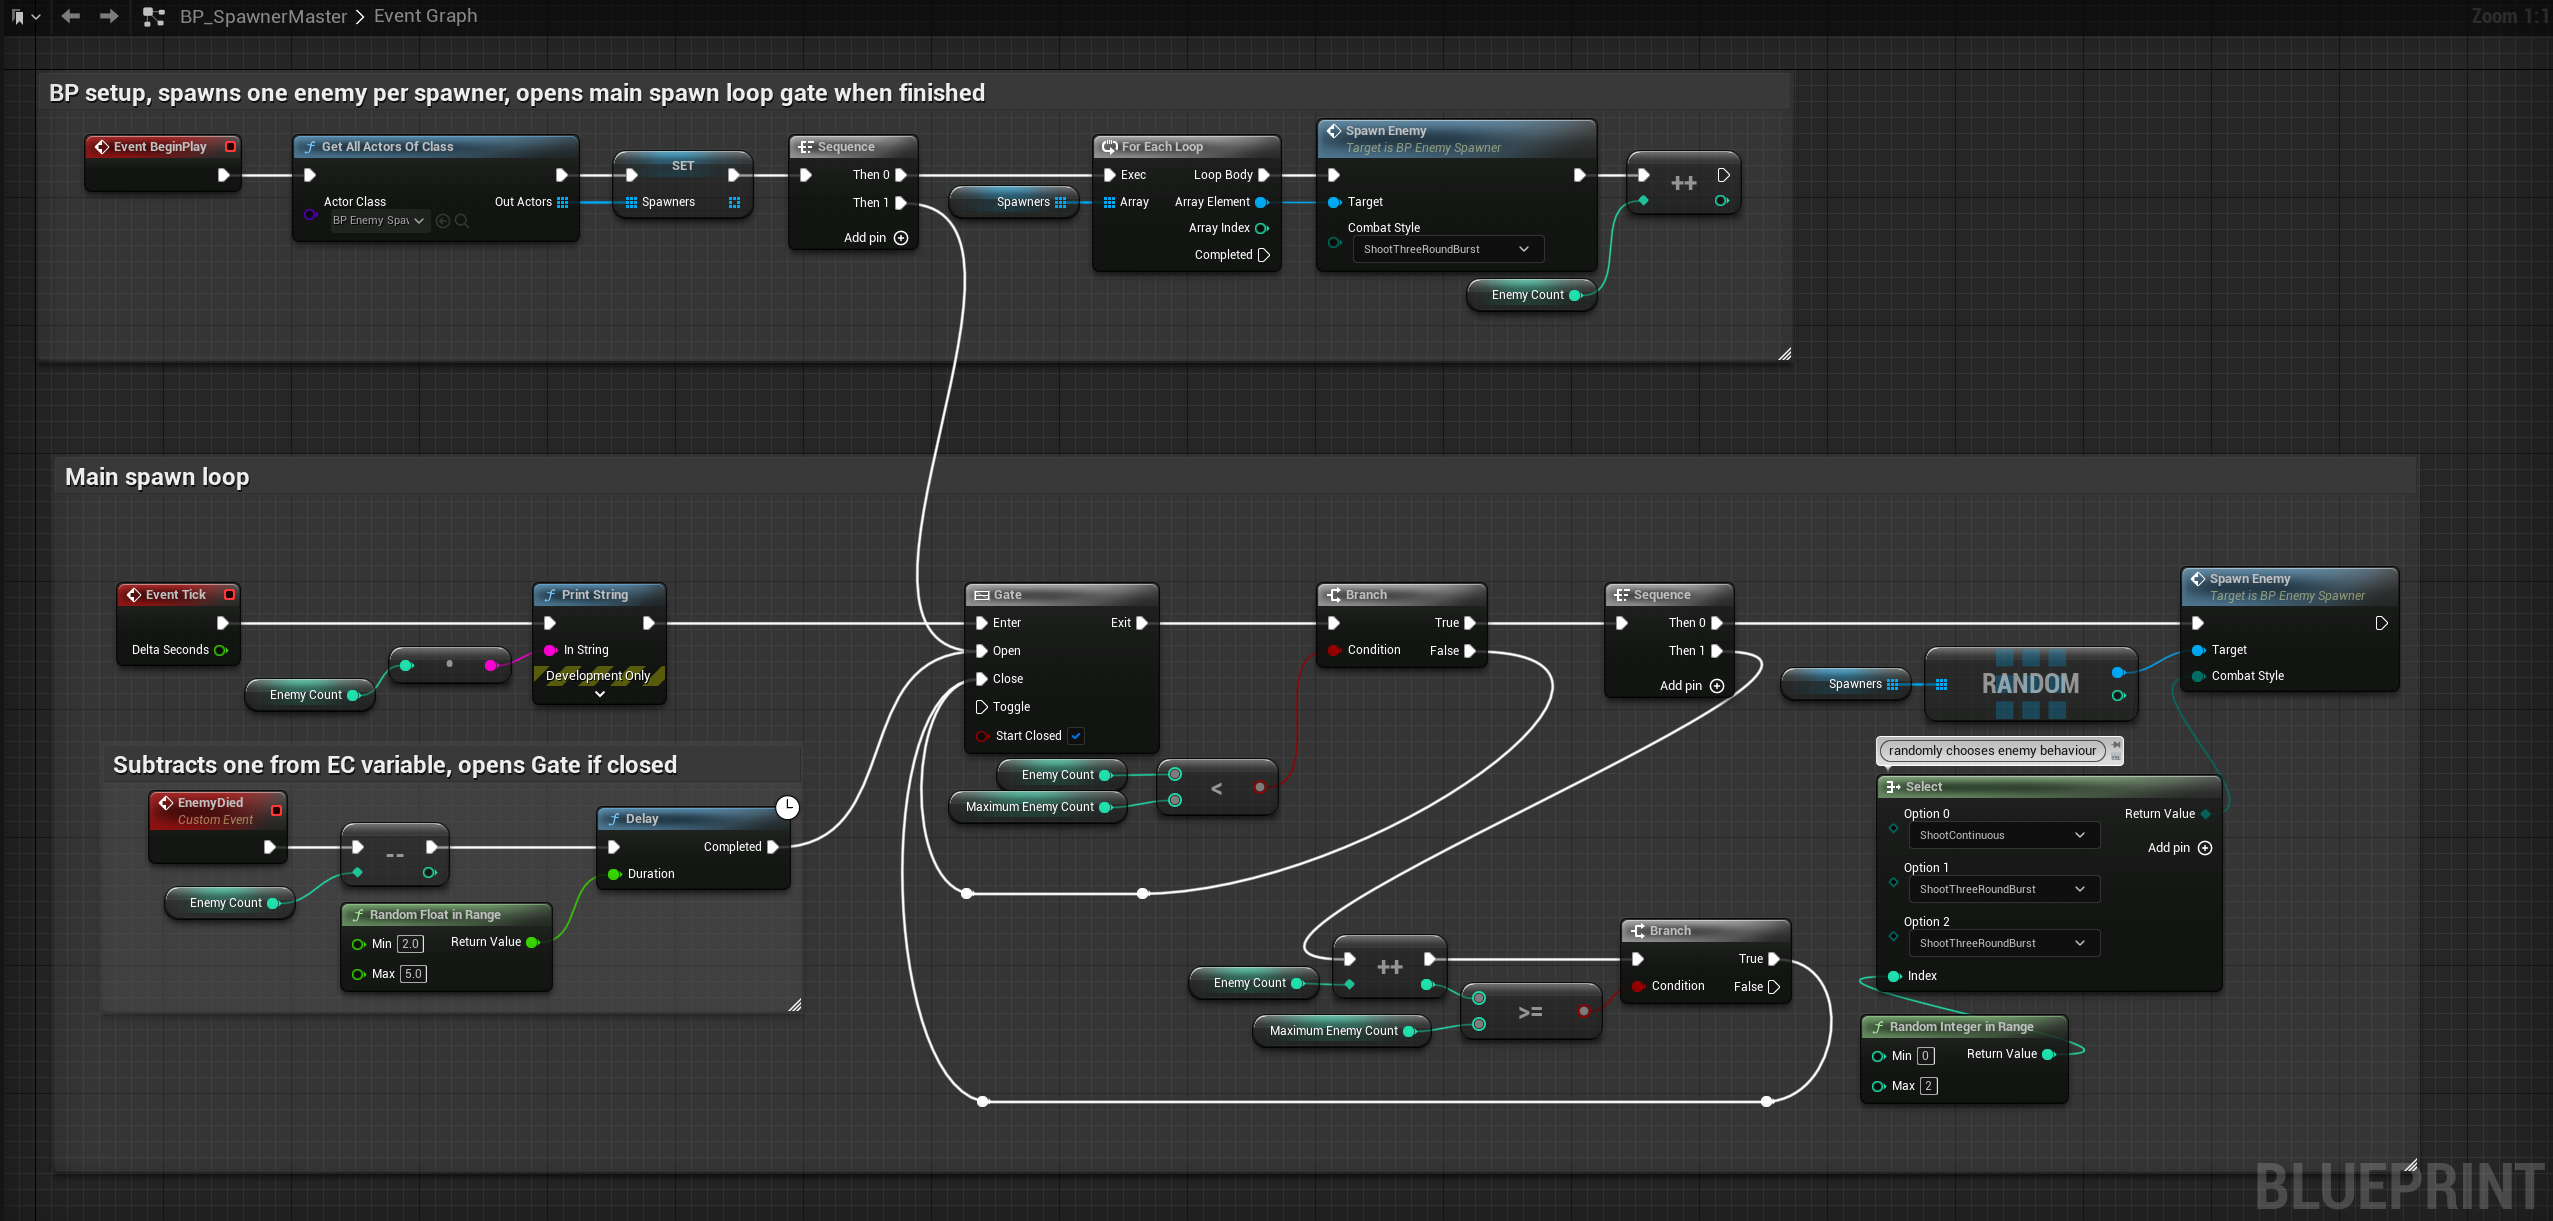
\includegraphics[width=1.0\linewidth]{images/masterspawner_nodesc.png}
\caption{\textit{BP{\_}MasterSpawner}, kód pro správu nepřátel}
\label{masterspawner}
\end{figure}
\clearpage

\begin{figure}[h!]
\centering
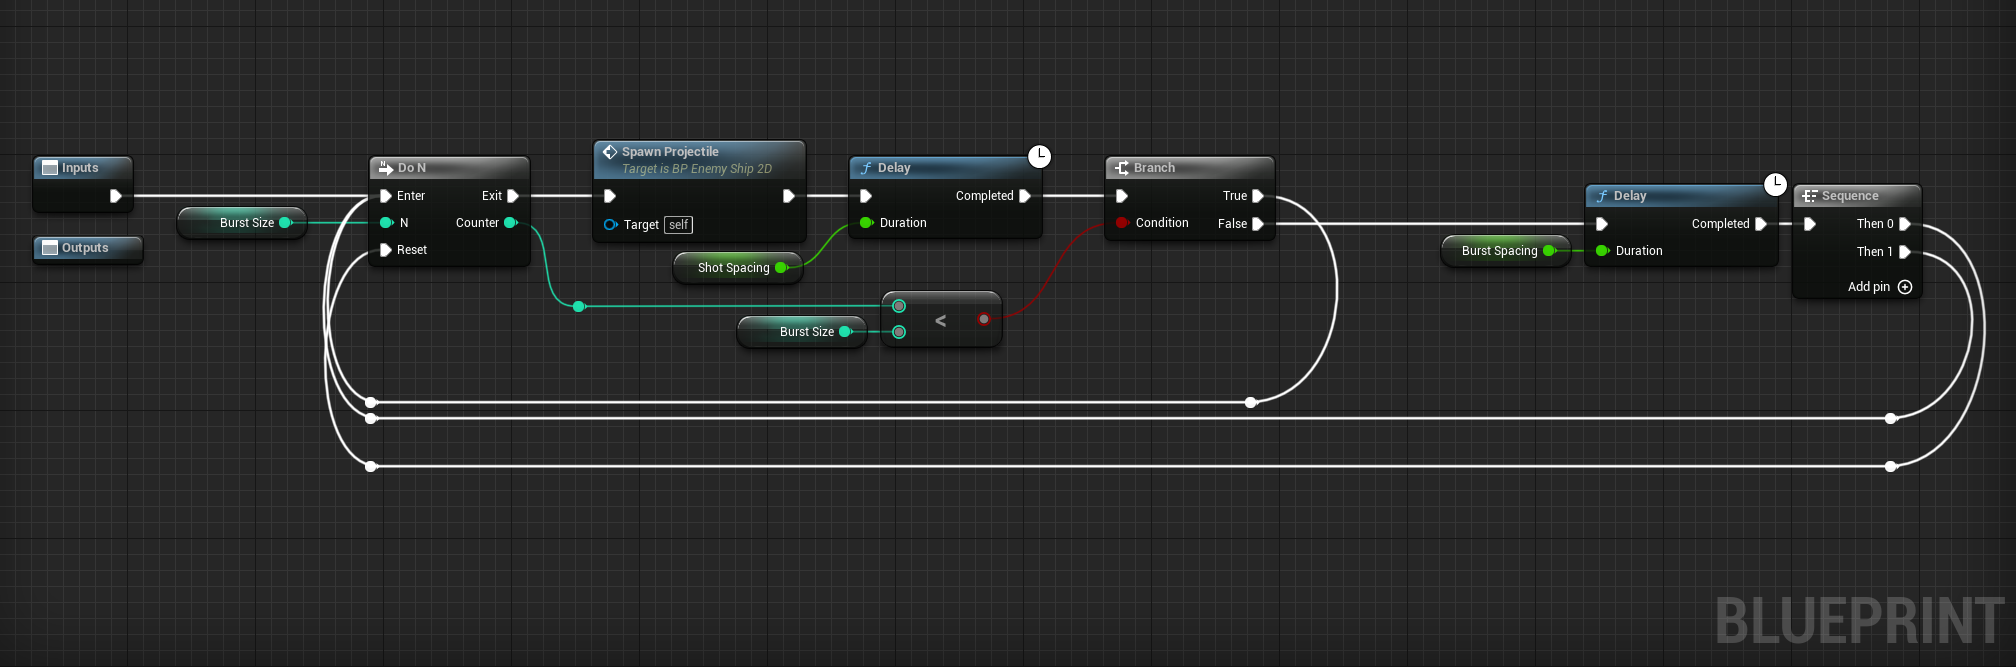
\includegraphics[width=1.0\linewidth]{images/shoot_burst.png}
\caption{Funkce \textit{ShootBurst}, která umožňuje střelbu v dávkách}
\label{burst}
\end{figure}
\clearpage
\end{landscape}

% BIBLIOGRAFIE, ZDROJE

\printbibliography
\addcontentsline{toc} {section} {Použitá literatura}

\end{document}